%%%%%%%%%%%%%%%%%%%%%%%%%%%%%%%%%%%%%%%%%
% Stylish Article
% LaTeX Template
% Version 2.1 (1/10/15)
%
% This template has been downloaded from:
% http://www.LaTeXTemplates.com
%
% Original author:
% Mathias Legrand (legrand.mathias@gmail.com) 
% With extensive modifications by:
% Vel (vel@latextemplates.com)
%
% License:
% CC BY-NC-SA 3.0 (http://creativecommons.org/licenses/by-nc-sa/3.0/)
%
%%%%%%%%%%%%%%%%%%%%%%%%%%%%%%%%%%%%%%%%%

%----------------------------------------------------------------------------------------
%	PACKAGES AND OTHER DOCUMENT CONFIGURATIONS
%----------------------------------------------------------------------------------------

\documentclass[fleqn,10pt]{SelfArx} % Document font size and equations flushed left

\usepackage[brazil]{babel} % Specify a different language here - english by default

\usepackage{lipsum} % Required to insert dummy text. To be removed otherwise

\usepackage[ruled,portuguese]{algorithm2e}

\usepackage{bchart}

\usepackage{mathtools}

\usepackage{changepage}

%----------------------------------------------------------------------------------------
%	COLUMNS
%----------------------------------------------------------------------------------------

\setlength{\columnsep}{0.55cm} % Distance between the two columns of text
\setlength{\fboxrule}{0.75pt} % Width of the border around the abstract

%----------------------------------------------------------------------------------------
%	COLORS
%----------------------------------------------------------------------------------------

\definecolor{color1}{RGB}{0,0,90} % Color of the article title and sections
\definecolor{color2}{RGB}{0,20,20} % Color of the boxes behind the abstract and headings

%----------------------------------------------------------------------------------------
%	HYPERLINKS
%----------------------------------------------------------------------------------------

\usepackage[hyphens]{url}
\usepackage{hyperref} % Required for hyperlinks
\hypersetup{hidelinks,colorlinks,breaklinks=true,urlcolor=color2,citecolor=color1,linkcolor=color1,bookmarksopen=false,pdftitle={Title},pdfauthor={Author}}

%----------------------------------------------------------------------------------------
%	ARTICLE INFORMATION
%----------------------------------------------------------------------------------------

\JournalInfo{Vitória,} % Journal information
\Archive{27 de Novembro, 2015} % Additional notes (e.g. copyright, DOI, review/research article) Vitória - ES, Brasil

\PaperTitle{Algoritmos de Ordenação} % Article title

\Authors{Vinicius Ferraço Arruda\textsuperscript{1}} % Authors
\affiliation{\textsuperscript{1}\textit{Departamento de Informática, Centro Tecnológico, Universidade Federal do Espírito Santo}} % Author affiliation
\affiliation{\textbf{E-mail}: viniciusferracoarruda@gmail.com} % Corresponding author

\Keywords{} % Keywords - if you don't want any simply remove all the text between the curly brackets
\newcommand{\keywordname}{Keywords} % Defines the keywords heading name

%----------------------------------------------------------------------------------------
%	ABSTRACT
%----------------------------------------------------------------------------------------

\Abstract{The purpose of this article is to show an analysis elaborated with 10 sorting algorithms. The analyzed algorithms 
were the bubble sort, shake sort, insertion sort, shell sort, selection sort, rank sort, merge sort, heap sort, radix sort
and quick sort where the radix sort has been implemented in two versions, one in decimal and other in binary and the quick 
sort in four versions, each version uses one of the following ways to select the pivot: the first element, the central 
element, the resulting element of the median of three and an element chosen randomly.

For each algorithm, a brief description of its operation is presented along with a chart showing the run-time of the 
algorithm.
The algorithms will sort sets of integers that compose a database.
The database is generated through an algorithm that generates integers in the closed interval [0, 1000000]. These numbers 
can be repeated, and can be generated in random, ascending and descending order.
Finally, a comparison between the algorithms was prepared indicating the most appropriate algorithms for each type of
order and number of values to be ordered.}


% O objetivo deste artigo é mostrar uma análise elaborada com 10 algoritmos de ordenação. Os algortmos analisados 
% foram o bubble sort, shake sort, insertion sort, shell sort, selection sort, rank sort, merge sort, heap sort, radix sort 
% e quick sort, onde, o radix sort foi implementado em duas versões, uma em decimal e outra binário, e o quick sort em quatro 
% versões, com escolha do pivô sendo o primeiro elemento, o elemento central, o elemento resultante do cálculo da mediana de
% três e um elemento aleatório.

% Para cada algoritmo, uma breve descrição de seu funcionamento é apresentada e a seguir um gráfico do tempo de execução 
% para ordenar um conjunto de números inteiros pertencente à base de dados gerada. A base de dados é gerada através de um 
% algoritmo que gera números inteiros no intervalo fechado [0, 1000000], esses números podem se repetir, e podem ser gerados 
% em ordem aleatória, crescente e descresente.
% Ao final, um comparativo entre os algoritmos foi elaborado, indicando os algoritmos mais adequados para cada base de dados.



%----------------------------------------------------------------------------------------

\begin{document}

\flushbottom % Makes all text pages the same height

\maketitle % Print the title and abstract box

\tableofcontents % Print the contents section

\thispagestyle{empty} % Removes page numbering from the first page

%----------------------------------------------------------------------------------------
%	ARTICLE CONTENTS
%----------------------------------------------------------------------------------------

\section{Introdução} % The \section*{} command stops section numbering

%\addcontentsline{toc}{section}{Introdução} % Adds this section to the table of contents

%\lipsum[1-3] Dummy text

Um algoritmo de ordenação é um algoritmo que coloca os elementos de uma lista em uma determidada ordem. As ordens mais 
utilizadas são as ordens numérica e lexicográfica. A ordenação eficiente é importante para otimizar o uso de outros 
algoritmos, como algoritmos de busca e de mistura (\emph{merge}), que requerem entrada de dados ordenada. É também 
útil para normalizar dados e para produzir dados mais legíveis para se interpretar e analisar.

Os dados a serem ordenados geralmente são dispostos em um \emph{array}, que permite acesso aleatório em tempo constante, 
em vez de listas, que permite apenas acesso sequencial, embora muitos algoritmos de ordenação podem ser modificados 
para se adequar a outros tipos de estrutura de dados.

Desde o início da computação, o problema de ordenação tem atraído um grande número de pesquisas, talvez devido 
à complexidade de resolvê-lo de forma eficiente, apesar de sua declaração simples e familiar.

Algoritmos de ordenação são frequentemente abordados nas aulas de ciência da computação, onde a abundância de algoritmos 
para o problema fornece uma introdução para uma variedade de conceitos fundamentais de algoritmos, como a notação O 
grande (\emph{big O notation}), algoritmos de dividir e conquistar, estruturas de dados, tais como pilhas e árvores 
binárias, análise de melhor, pior e médio caso, permutação entre tempo de execução e espaço de armazenamento 
(\emph{space-time tradeoff}) e limites superiores e inferiores [\ref{SortAlgoWiki}].


%------------------------------------------------

\section{Metodologia}

Inicialmente, foi elaborado um algoritmo para gerar números inteiros para compor a base de testes dos algoritmos de 
ordenação. Este algoritmo gera uma sequência de números inteiros em ordem aleatória, crescente e decrescente, podendo 
haver números repetidos.

Os algoritmos de ordenação implementados foram o bubble sort, shake sort, insertion sort, shell sort, selection sort, 
rank sort, merge sort, heap sort, radix sort e quick sort, onde o radix sort possue duas versões e o quick sort 
quatro versões. 

%------------------------------------------------

\section{Ferramentas}

Os algoritmos foram implementados utilizando a linguagem de programação C seguindo o padrão C90 e 
compilados utilizando o compilador GCC versão 4.8.4. Para auxiliar na depuração dos códigos foi utilizado o 
programa Valgrind versão 3.10.0. 

Os algoritmos foram implementados e executados em uma máquina com sistema operacional Ubuntu versão 14.04.3, 
arquitetura 64 bits, CPU Intel i7-5500U 2.40GHz, 16 Gib de memória RAM DDR3L.

%------------------------------------------------

\section{Base de Testes}

A base de testes foi gerada utilizando um algoritmo elaborado para gerar \emph{n} números inteiros aleatórios no intervalo 
[0, 1.000.000]. Três versões deste algoritmo foi implementado, gerando números em ordem aleatória, crescente e descresente.

Para a implementação, foi utilizado para gerar números aleatórios a função \emph{srand()} e \emph{rand()} da biblioteca 
padrão de C (\emph{stdlib}). Também desta mesma biblioteca, foi utilizado para implementar as versões crescente e 
decrescente a função \emph{qsort()}.

A base de testes está dividida em três sub-bases com ordens distintas: aleatória, crescente e decrescente. 
Cada sub-base possui 7 arquivos, contendo 10\textsuperscript{2}, 10\textsuperscript{3}, 10\textsuperscript{4}, 
10\textsuperscript{5}, 10\textsuperscript{6}, 10\textsuperscript{7}, 10\textsuperscript{8} números inteiros,
respectivamente.  

Todos os algoritmos foram submetidos à esta base de testes. Os algoritmos que não executaram com algum arquivo da base de 
testes em até 65 minutos tiveram sua execução interrompida e o resultado para este arquivo foi omitido.

%------------------------------------------------

\section{Algoritmos de Ordenação}

\subsection{Bubble Sort}

O bubble sort é geralmente considerado o mais simples algoritmo de ordenação. Devido à sua simplicidade e facilidade 
de visualização, muitas vezes é ensinada em cursos introdutórios de ciência da computação. Por causa de seu
desempenho O(n\textsuperscript{2}), ele não é utilizado para grandes (ou mesmo médios) conjuntos de dados.

O bubble sort funciona passando sequencialmente sobre um vetor, comparando cada elemento com o imediatamente após ele. Se 
o primeiro elemento for maior que o segundo (considerando a ordem crescente como desejada), as suas posições são comutadas. 

Ao longo de um número de passagens, no máximo igual ao número de elementos do vetor, todos os valores vão para as suas 
posições corretas, pois cada passagem encontra o maior elemento e o coloca na extremidade do vetor. A porção do vetor a ser 
ordenada pode ser reduzida em cada passagem. Uma variável auxiliar é utilizada para controlar se houve alterações 
na passagem corrente. Depois de uma passagem completa sem nenhuma alteração no vetor, o algoritmo é encerrado.

\subsubsection*{Resultados}

A seguir os gráficos do tempo da execução do algoritmo bubble sort com a base de testes:\newline

{\setlength{\parindent}{-0.5em}
\scalebox{0.9}{
\begin{bchart}[max=3614, plain, scale=0.9, unit=s]
\bcbar[label=10\textsuperscript{2}]{0.000}
\bcbar[label=10\textsuperscript{3}]{0.007}
\bcbar[label=10\textsuperscript{4}]{0.282}
\bcbar[label=10\textsuperscript{5}]{33.513}
\bcbar[label=10\textsuperscript{6}]{3613.248}
\bcxlabel{Ordem aleatória}
\end{bchart}}}\newline

{\setlength{\parindent}{-0.5em}
\scalebox{0.9}{
\begin{bchart}[max=11, plain, scale=0.9, unit=s]
\bcbar[label=10\textsuperscript{2}]{0.000}
\bcbar[label=10\textsuperscript{3}]{0.000}
\bcbar[label=10\textsuperscript{4}]{0.000}
\bcbar[label=10\textsuperscript{5}]{0.010}
\bcbar[label=10\textsuperscript{6}]{0.094}
\bcbar[label=10\textsuperscript{7}]{0.929}
\bcbar[label=10\textsuperscript{8}]{10.522}
\bcxlabel{Ordem crescente}
\end{bchart}}}\newline

{\setlength{\parindent}{-0.5em}
\scalebox{0.9}{
\begin{bchart}[max=2855, plain, scale=0.9, unit=s]
\bcbar[label=10\textsuperscript{2}]{0.000}
\bcbar[label=10\textsuperscript{3}]{0.003}
\bcbar[label=10\textsuperscript{4}]{0.246}
\bcbar[label=10\textsuperscript{5}]{25.738}
\bcbar[label=10\textsuperscript{6}]{2854.567}
\bcxlabel{Ordem decrescente}
\end{bchart}}}\newline

O bubble sort possui um melhor caso, que é de complexidade \emph{O(n)}, e ele ocorre quando todos os elementos já estão 
ordenados, passando somente uma única vez pelo vetor. Podemos observar este resultado no gráfico da base de testes 
ordenada, onde o tempo de execução foi muito menor que os das bases de testes aleatória e decrescente. Para estas duas 
bases, os testes com 10\textsuperscript{7} e 10\textsuperscript{8} números inteiros tiveram suas execuções interrompidas 
devido ao longo tempo de execução, tendo seus dados omitidos nos gráficos acima.

\subsection{Shake Sort}

O shake sort é um aperfeiçoamento do algoritmo bubble sort, considerando uma ordenação em ordem crescente, ao final de uma 
varredura da esquerda para a direita, o funcionamento é identico ao bubble sort, colocando o maior elemento ao final do 
vetor. O incremento é feito ao chegar no final do vetor, efetuando uma varredura da direita para a esquerda, colocando o 
menor elemento no início do vetor.

\subsubsection*{Resultados}

A seguir os gráficos do tempo da execução do algoritmo shake sort com a base de testes:\newline

{\setlength{\parindent}{-0.5em}
\scalebox{0.9}{
\begin{bchart}[max=2659, plain, scale=0.9, unit=s]
\bcbar[label=10\textsuperscript{2}]{0.001}
\bcbar[label=10\textsuperscript{3}]{0.006}
\bcbar[label=10\textsuperscript{4}]{0.216}
\bcbar[label=10\textsuperscript{5}]{27.867}
\bcbar[label=10\textsuperscript{6}]{2658.173}
\bcxlabel{Ordem aleatória}
\end{bchart}}}\newline

{\setlength{\parindent}{-0.5em}
\scalebox{0.9}{
\begin{bchart}[max=10, plain, scale=0.9, unit=s]
\bcbar[label=10\textsuperscript{2}]{0.000}
\bcbar[label=10\textsuperscript{3}]{0.000}
\bcbar[label=10\textsuperscript{4}]{0.003}
\bcbar[label=10\textsuperscript{5}]{0.022}
\bcbar[label=10\textsuperscript{6}]{0.209}
\bcbar[label=10\textsuperscript{7}]{1.730}
\bcbar[label=10\textsuperscript{8}]{9.908}
\bcxlabel{Ordem crescente}
\end{bchart}}}\newline

{\setlength{\parindent}{-0.5em}
\scalebox{0.9}{
\begin{bchart}[max=2768, plain, scale=0.9, unit=s]
\bcbar[label=10\textsuperscript{2}]{0.000}
\bcbar[label=10\textsuperscript{3}]{0.000}
\bcbar[label=10\textsuperscript{4}]{0.236}
\bcbar[label=10\textsuperscript{5}]{33.215}
\bcbar[label=10\textsuperscript{6}]{2767.370}
\bcxlabel{Ordem decrescente}
\end{bchart}}}\newline

O shake sort, por mais que tenha um incremento em relação ao bubble sort, ainda possui complexidade 
\emph{O(n\textsuperscript{2})} e a diferença de tempo de execução entre o bubble e o shake sort é mínima. O shake sort 
tem como melhor caso, assim como o bubble sort, quando executado sobre uma base já ordenada, a complexidade \emph{O(n)}.
Os dados das bases com ordem aleatória e decrescente com 10\textsuperscript{7} e 10\textsuperscript{8} números inteiros 
foram omitidos, pois tiveram suas execuções interrompidas devido ao longo tempo de execução.

\subsection{Insertion Sort}

Insertion sort, ou ordenação por inserção, é um simples algoritmo de ordenação, que percorre um vetor de elementos da 
esquerda para a direita e à medida que avança vai deixando os elementos mais à esquerda ordenados. O insertion sort tem 
como complexidade O(n\textsuperscript{2}), e é indicado para ordenar pequenos números de elementos e quando se tem dados 
parcialmente ordenados.

\subsubsection*{Resultados}

A seguir os gráficos do tempo da execução do algoritmo insertion sort com a base de testes:\newline

{\setlength{\parindent}{-0.5em}
\scalebox{0.9}{
\begin{bchart}[max=966, plain, scale=0.9, unit=s]
\bcbar[label=10\textsuperscript{2}]{0.000}
\bcbar[label=10\textsuperscript{3}]{0.005}
\bcbar[label=10\textsuperscript{4}]{0.087}
\bcbar[label=10\textsuperscript{5}]{8.637}
\bcbar[label=10\textsuperscript{6}]{965.882}
\bcxlabel{Ordem aleatória}
\end{bchart}}}\newline

{\setlength{\parindent}{-0.5em}
\scalebox{0.9}{
\begin{bchart}[max=17, plain, scale=0.9, unit=s]
\bcbar[label=10\textsuperscript{2}]{0.000}
\bcbar[label=10\textsuperscript{3}]{0.000}
\bcbar[label=10\textsuperscript{4}]{0.002}
\bcbar[label=10\textsuperscript{5}]{0.017}
\bcbar[label=10\textsuperscript{6}]{0.162}
\bcbar[label=10\textsuperscript{7}]{1.642}
\bcbar[label=10\textsuperscript{8}]{16.432}
\bcxlabel{Ordem crescente}
\end{bchart}}}\newline

{\setlength{\parindent}{-0.5em}
\scalebox{0.9}{
\begin{bchart}[max=1843, plain, scale=0.9, unit=s]
\bcbar[label=10\textsuperscript{2}]{0.000}
\bcbar[label=10\textsuperscript{3}]{0.000}
\bcbar[label=10\textsuperscript{4}]{0.166}
\bcbar[label=10\textsuperscript{5}]{21.857}
\bcbar[label=10\textsuperscript{6}]{1842.664}
\bcxlabel{Ordem decrescente}
\end{bchart}}}\newline

No melhor caso, o insertion sort possui complexidade \emph{O(n)}, e ocorre quando os elementos já estão ordenados, como 
mostra os dados acima com a base de testes em ordem crescente. Os dados de 10\textsuperscript{7} e 
10\textsuperscript{8} números inteiros das bases de testes com ordem aleatória e crescente foram omitidos devido 
a demora para completar sua execução.

\subsection{Shell Sort}

Criado por Donald Shell em 1959, o shell sort é o mais eficiente algoritmo de ordenação dentre os de complexidade 
quadrática. É um refinamento do algoritmo insertion sort. O algoritmo difere do insertion sort pelo fato de no lugar de 
considerar o vetor a ser ordenado como um único segmento, ele considera vários segmentos sendo aplicado o algoritmo 
insertion sort em cada um deles. Basicamente o algoritmo passa várias vezes pelo vetor dividindo o grupo maior em grupos 
menores. Nos grupos menores é aplicado o insertion sort.

\subsubsection*{Resultados}

A seguir os gráficos do tempo da execução do algoritmo shell sort com a base de testes:\newline

{\setlength{\parindent}{-0.5em}
\scalebox{0.9}{
\begin{bchart}[max=104, plain, scale=0.9, unit=s]
\bcbar[label=10\textsuperscript{2}]{0.000}
\bcbar[label=10\textsuperscript{3}]{0.000}
\bcbar[label=10\textsuperscript{4}]{0.004}
\bcbar[label=10\textsuperscript{5}]{0.039}
\bcbar[label=10\textsuperscript{6}]{0.476}
\bcbar[label=10\textsuperscript{7}]{6.828}
\bcbar[label=10\textsuperscript{8}]{103.221}
\bcxlabel{Ordem aleatória}
\end{bchart}}}\newline

{\setlength{\parindent}{-0.5em}
\scalebox{0.9}{
\begin{bchart}[max=25, plain, scale=0.9, unit=s]
\bcbar[label=10\textsuperscript{2}]{0.000}
\bcbar[label=10\textsuperscript{3}]{0.000}
\bcbar[label=10\textsuperscript{4}]{0.003}
\bcbar[label=10\textsuperscript{5}]{0.030}
\bcbar[label=10\textsuperscript{6}]{0.308}
\bcbar[label=10\textsuperscript{7}]{3.309}
\bcbar[label=10\textsuperscript{8}]{24.087}
\bcxlabel{Ordem crescente}
\end{bchart}}}\newline

{\setlength{\parindent}{-0.5em}
\scalebox{0.9}{
\begin{bchart}[max=36, plain, scale=0.9, unit=s]
\bcbar[label=10\textsuperscript{2}]{0.000}
\bcbar[label=10\textsuperscript{3}]{0.000}
\bcbar[label=10\textsuperscript{4}]{0.000}
\bcbar[label=10\textsuperscript{5}]{0.019}
\bcbar[label=10\textsuperscript{6}]{0.202}
\bcbar[label=10\textsuperscript{7}]{2.275}
\bcbar[label=10\textsuperscript{8}]{35.869}
\bcxlabel{Ordem decrescente}
\end{bchart}}}\newline

O algoritmo shell sort se mostrou muito mais eficiente que os outros algoritmos de complexidade quadrática, executando 
todas as bases de testes em um tempo muito inferior. Porém é um algoritmo que depende dos valores de 
entrada\footnote{Em [\ref{ShellWiki}], no capitulo \emph{Gap sequences}, há um comparativo de escolhas de intervalo a se 
dividir o vetor, mostrando a complexidade do pior caso para cada intervalo. Para este artigo, foi utilizado o 
intervalo $\lfloor n/2\textsuperscript{k} \rfloor$, que possui complexidade \emph{O(n\textsuperscript{2})} no pior caso.},
 tendo como melhor e pior caso as complexidades \emph{O(n $\log_2$n)} e \emph{O(n\textsuperscript{2})}, respectivamente.

\subsection{Selection Sort}

O algoritmo selection sort divide o vetor de entrada em duas partes: o sub-vetor de itens já ordenados, e o sub-vetor de 
itens a serem ordenados que ocupam o resto do vetor. Inicialmente, o sub-vetor ordenado está vazio e o sub-vetor 
não ordenado é o vetor inteiro de entrada. O algoritmo prossegue encontrando o menor (ou maior, dependendo da ordem de 
ordenação) elemento no sub-vetor dos não ordenados, comutando com o elemento mais à esquerda dos não ordenados, colocando-o 
em sua posição ordenada, e incrementando o limite do sub-vetor de elementos ordenados um elemento para a direita.

\subsubsection*{Resultados}

A seguir os gráficos do tempo da execução do algoritmo selection sort com a base de testes:\newline

{\setlength{\parindent}{-0.5em}
\scalebox{0.9}{
\begin{bchart}[max=1658, plain, scale=0.9, unit=s]
\bcbar[label=10\textsuperscript{2}]{0.000}
\bcbar[label=10\textsuperscript{3}]{0.005}
\bcbar[label=10\textsuperscript{4}]{0.148}
\bcbar[label=10\textsuperscript{5}]{15.512}
\bcbar[label=10\textsuperscript{6}]{1657.082}
\bcxlabel{Ordem aleatória}
\end{bchart}}}\newline

{\setlength{\parindent}{-0.5em}
\scalebox{0.9}{
\begin{bchart}[max=2077, plain, scale=0.9, unit=s]
\bcbar[label=10\textsuperscript{2}]{0.000}
\bcbar[label=10\textsuperscript{3}]{0.000}
\bcbar[label=10\textsuperscript{4}]{0.189}
\bcbar[label=10\textsuperscript{5}]{17.053}
\bcbar[label=10\textsuperscript{6}]{2076.970}
\bcxlabel{Ordem crescente}
\end{bchart}}}\newline

{\setlength{\parindent}{-0.5em}
\scalebox{0.9}{
\begin{bchart}[max=3589, plain, scale=0.9, unit=s]
\bcbar[label=10\textsuperscript{2}]{0.000}
\bcbar[label=10\textsuperscript{3}]{0.002}
\bcbar[label=10\textsuperscript{4}]{0.140}
\bcbar[label=10\textsuperscript{5}]{16.885}
\bcbar[label=10\textsuperscript{6}]{3588.222}
\bcxlabel{Ordem decrescente}
\end{bchart}}}\newline

O selecion sort, independente da entrada, possui complexidade para qualquer caso de \emph{O(n\textsuperscript{2})}. 
Os tempos de execução de todas as bases com 10\textsuperscript{7} e 10\textsuperscript{8} números inteiros foi grande 
demais e tiveram suas execuções interrompidas e seus dados nos gráficos omitidos.

\subsection{Rank Sort}

O algoritmo rank sort, ou counting sort, funciona percorrendo o vetor a ser ordenado contando quantas vezes um 
determinado elemento aparece e armazenando essa contagem em um vetor auxiliar de tamanho igual ao maior elemento do vetor 
mais um na posição do valor do elemento. Ao fim da contagem, o vetor ordenado é montado a partir do vetor auxiliar, 
percorrendo em ordem crescente (supondo ordem crescente) e inserindo no vetor ordenado o valor do índice do elemento do 
vetor auxiliar, onde este elemento é o número de vezes que o elemento com o valor deste índice aparece no vetor. O valor do 
índice é inserido o número de vezes que este valor se encontra no vetor.

\subsubsection*{Resultados}

A seguir os gráficos do tempo da execução do algoritmo rank sort com a base de testes:\newline

{\setlength{\parindent}{-0.5em}
\scalebox{0.9}{
\begin{bchart}[max=11, plain, scale=0.9, unit=s]
\bcbar[label=10\textsuperscript{2}]{0.003}
\bcbar[label=10\textsuperscript{3}]{0.006}
\bcbar[label=10\textsuperscript{4}]{0.008}
\bcbar[label=10\textsuperscript{5}]{0.022}
\bcbar[label=10\textsuperscript{6}]{0.117}
\bcbar[label=10\textsuperscript{7}]{1.020}
\bcbar[label=10\textsuperscript{8}]{10.754}
\bcxlabel{Ordem aleatória}
\end{bchart}}}\newline

{\setlength{\parindent}{-0.5em}
\scalebox{0.9}{
\begin{bchart}[max=11, plain, scale=0.9, unit=s]
\bcbar[label=10\textsuperscript{2}]{0.000}
\bcbar[label=10\textsuperscript{3}]{0.004}
\bcbar[label=10\textsuperscript{4}]{0.005}
\bcbar[label=10\textsuperscript{5}]{0.015}
\bcbar[label=10\textsuperscript{6}]{0.111}
\bcbar[label=10\textsuperscript{7}]{0.980}
\bcbar[label=10\textsuperscript{8}]{10.251}
\bcxlabel{Ordem crescente}
\end{bchart}}}\newline

{\setlength{\parindent}{-0.5em}
\scalebox{0.9}{
\begin{bchart}[max=10, plain, scale=0.9, unit=s]
\bcbar[label=10\textsuperscript{2}]{0.005}
\bcbar[label=10\textsuperscript{3}]{0.006}
\bcbar[label=10\textsuperscript{4}]{0.008}
\bcbar[label=10\textsuperscript{5}]{0.018}
\bcbar[label=10\textsuperscript{6}]{0.112}
\bcbar[label=10\textsuperscript{7}]{1.067}
\bcbar[label=10\textsuperscript{8}]{9.663}
\bcxlabel{Ordem decrescente}
\end{bchart}}}\newline

O algoritmo rank sort, dentre todos os algoritmos deste artigo, obteve os melhores resultados. Isso se deve à sua 
complexidade \emph{O(n + k)} para todos os casos, onde \emph{n} é o número de inteiros à ser ordenado e \emph{k} é 
o valor do maior número inteiro contido na base a ser ordenada. A desvantagem deste algoritmo é que tem como 
espaço de uso \emph{O(n + k)}, pois o vetor a ser ordenado possui comprimento \emph{n} e o vetor auxiliar para 
a contagem possui comprimento \emph{k + 1}. O rank sort está restrito à problemas onde os elementos a serem 
ordenados sejam dados discretos, pois são utilizados como índices de memória.

\subsection{Merge Sort}

O algoritmo merge sort foi inventado em 1945 por John von Neumann, e possui complexidade \emph{O(n $\log_2$n)}. 
O merge sort é um algoritmo recursivo que segue a idéia simples de dividir e conquistar. Primeiro o vetor de elementos é 
dividido em grupos pequenos recursivamente, até que tenham apenas um ou nenhum elemento, que já estão ordenados. Em 
seguida, retornando a recursão, os elementos são mesclados formando pequenos vetores ordenados. A medida que a pilha de 
recursão vai se desfazendo, esses pequenos vetores ordenados vão se mesclando de maneira ordenada.

\subsubsection*{Resultados}

A seguir os gráficos do tempo da execução do algoritmo merge sort com a base de testes:\newline

{\setlength{\parindent}{-0.5em}
\scalebox{0.9}{
\begin{bchart}[max=61, plain, scale=0.9, unit=s]
\bcbar[label=10\textsuperscript{2}]{0.000}
\bcbar[label=10\textsuperscript{3}]{0.000}
\bcbar[label=10\textsuperscript{4}]{0.004}
\bcbar[label=10\textsuperscript{5}]{0.034}
\bcbar[label=10\textsuperscript{6}]{0.357}
\bcbar[label=10\textsuperscript{7}]{4.085}
\bcbar[label=10\textsuperscript{8}]{60.310}
\bcxlabel{Ordem aleatória}
\end{bchart}}}\newline

{\setlength{\parindent}{-0.5em}
\scalebox{0.9}{
\begin{bchart}[max=48, plain, scale=0.9, unit=s]
\bcbar[label=10\textsuperscript{2}]{0.000}
\bcbar[label=10\textsuperscript{3}]{0.000}
\bcbar[label=10\textsuperscript{4}]{0.004}
\bcbar[label=10\textsuperscript{5}]{0.028}
\bcbar[label=10\textsuperscript{6}]{0.238}
\bcbar[label=10\textsuperscript{7}]{2.527}
\bcbar[label=10\textsuperscript{8}]{47.257}
\bcxlabel{Ordem crescente}
\end{bchart}}}\newline

{\setlength{\parindent}{-0.5em}
\scalebox{0.9}{
\begin{bchart}[max=51, plain, scale=0.9, unit=s]
\bcbar[label=10\textsuperscript{2}]{0.000}
\bcbar[label=10\textsuperscript{3}]{0.000}
\bcbar[label=10\textsuperscript{4}]{0.005}
\bcbar[label=10\textsuperscript{5}]{0.042}
\bcbar[label=10\textsuperscript{6}]{0.446}
\bcbar[label=10\textsuperscript{7}]{4.476}
\bcbar[label=10\textsuperscript{8}]{50.882}
\bcxlabel{Ordem decrescente}
\end{bchart}}}\newline

O algoritmo merge sort, possui complexidade constante e tem como desvantagem o uso do dobro de memória,
 pois necessita de uma vetor de comprimeito \emph{n} para armazenar os valores a serem ordenados e outros vetores que 
 serão necessários ao longo da execução do algoritmo, que possuem comprimento \emph{n} ao serem somados. Uma outra 
 desvantagem do merge sort é o fato de ser um algoritmo recursivo, tendo um empilhamento de \emph{$\log_2$n + 1} 
 chamadas ao algoritmo merge sort\footnote{Isto é, a árvore de recursão do algoritmo merge sort possui profundidade 
 \emph{$\log_2$n + 1}.}.

\subsection{Quick Sort}

O algoritmo quick sort, criado por C.A.R. Hoare em 1960, adota a estratégia de divisão e conquista. A estratégia consiste 
em rearranjar os elementos de modo que os elementos menores precedam os elementos maiores (supondo uma ordem crescente dos 
elementos). Em seguida o quick sort ordena os dois sub-vetores de elementos menores e maiores 
recursivamente até que o vetor completo se encontre ordenado.

Os passos para a execução do quick sort são:
\begin{enumerate}
	\item Escolha um elemento do vetor, denominado pivô.

	\item Rearranje o vetor de forma que todos os elementos anteriores ao pivô sejam menores que ele, e todos os elementos
	 posteriores ao pivô sejam maiores que ele. Ao fim do processo o pivô estará em sua posição final e haverá dois sub-
	 vetores não ordenados. Essa operação é denominada partição.
	
	\item Recursivamente ordene o sub-vetor dos elementos menores e o sub-vetor dos elementos maiores.
\end{enumerate}
A base da recursão são os vetores de tamanho zero ou um, que estão sempre ordenados. O processo é finito, pois a cada 
iteração pelo menos um elemento é posto em sua posição final e não será mais manipulado na iteração seguinte.

Para uma melhor análise do quick sort, o passo 1 foi feito de quatro formas distintas, escolhendo como pivô o primeiro 
elemento, o elemento central, um elemento escolhido aleatoriamente e o elemento resultante da mediana de três, onde os três 
elementos escolhidos são o primeiro, o central e o último.

\subsubsection*{Primeiro elemento}

A seguir os gráficos do tempo da execução do algoritmo quick sort com a base de testes, com o pivô sendo o 
primeiro elemento:\newline

{\setlength{\parindent}{-0.5em}
\scalebox{0.9}{
\begin{bchart}[max=60, plain, scale=0.9, unit=s]
\bcbar[label=10\textsuperscript{2}]{0.000}
\bcbar[label=10\textsuperscript{3}]{0.000}
\bcbar[label=10\textsuperscript{4}]{0.002}
\bcbar[label=10\textsuperscript{5}]{0.025}
\bcbar[label=10\textsuperscript{6}]{0.254}
\bcbar[label=10\textsuperscript{7}]{2.688}
\bcbar[label=10\textsuperscript{8}]{59.992}
\bcxlabel{Ordem aleatória}
\end{bchart}}}\newline

%c1000000;runC: linha 11: 12245 Falha de segmentação  (imagem do núcleo gravada) ../../trab4 $algorithm $i < ../c$i.txt
%comentar da falha de segmentação stack overflow.

{\setlength{\parindent}{-0.5em}
\scalebox{0.9}{
\begin{bchart}[max=13, plain, scale=0.9, unit=s]
\bcbar[label=10\textsuperscript{2}]{0.000}
\bcbar[label=10\textsuperscript{3}]{0.000}
\bcbar[label=10\textsuperscript{4}]{0.127}
\bcbar[label=10\textsuperscript{5}]{12.897}
\bcxlabel{Ordem crescente}
\end{bchart}}}\newline

%d1000000;runD: linha 11: 12249 Falha de segmentação  (imagem do núcleo gravada) ../../trab4 $algorithm $i < ../d$i.txt
%comentar da falha de segmentação stack overflow.

{\setlength{\parindent}{-0.5em}
\scalebox{0.9}{
\begin{bchart}[max=14, plain, scale=0.9, unit=s]
\bcbar[label=10\textsuperscript{2}]{0.000}
\bcbar[label=10\textsuperscript{3}]{0.000}
\bcbar[label=10\textsuperscript{4}]{0.158}
\bcbar[label=10\textsuperscript{5}]{13.959}
\bcxlabel{Ordem decrescente}
\end{bchart}}}

\subsubsection*{Elemento central}

A seguir os gráficos do tempo da execução do algoritmo quick sort com a base de testes, com o pivô sendo o 
elemento central:\newline

{\setlength{\parindent}{-0.5em}
\scalebox{0.9}{
\begin{bchart}[max=57, plain, scale=0.9, unit=s]
\bcbar[label=10\textsuperscript{2}]{0.000}
\bcbar[label=10\textsuperscript{3}]{0.000}
\bcbar[label=10\textsuperscript{4}]{0.005}
\bcbar[label=10\textsuperscript{5}]{0.034}
\bcbar[label=10\textsuperscript{6}]{0.249}
\bcbar[label=10\textsuperscript{7}]{2.674}
\bcbar[label=10\textsuperscript{8}]{56.944}
\bcxlabel{Ordem aleatória}
\end{bchart}}}\newline

{\setlength{\parindent}{-0.5em}
\scalebox{0.9}{
\begin{bchart}[max=46, plain, scale=0.9, unit=s]
\bcbar[label=10\textsuperscript{2}]{0.000}
\bcbar[label=10\textsuperscript{3}]{0.000}
\bcbar[label=10\textsuperscript{4}]{0.000}
\bcbar[label=10\textsuperscript{5}]{0.012}
\bcbar[label=10\textsuperscript{6}]{0.159}
\bcbar[label=10\textsuperscript{7}]{1.750}
\bcbar[label=10\textsuperscript{8}]{45.002}
\bcxlabel{Ordem crescente}
\end{bchart}}}\newline

{\setlength{\parindent}{-0.5em}
\scalebox{0.9}{
\begin{bchart}[max=52, plain, scale=0.9, unit=s]
\bcbar[label=10\textsuperscript{2}]{0.000}
\bcbar[label=10\textsuperscript{3}]{0.000}
\bcbar[label=10\textsuperscript{4}]{0.003}
\bcbar[label=10\textsuperscript{5}]{0.027}
\bcbar[label=10\textsuperscript{6}]{0.271}
\bcbar[label=10\textsuperscript{7}]{2.915}
\bcbar[label=10\textsuperscript{8}]{51.404}
\bcxlabel{Ordem decrescente}
\end{bchart}}}

\subsubsection*{Elemento aleatório}

A seguir os gráficos do tempo da execução do algoritmo quick sort com a base de testes, com o pivô sendo um  
elemento aleatório:\newline

{\setlength{\parindent}{-0.5em}
\scalebox{0.9}{
\begin{bchart}[max=60, plain, scale=0.9, unit=s]
\bcbar[label=10\textsuperscript{2}]{0.000}
\bcbar[label=10\textsuperscript{3}]{0.000}
\bcbar[label=10\textsuperscript{4}]{0.004}
\bcbar[label=10\textsuperscript{5}]{0.034}
\bcbar[label=10\textsuperscript{6}]{0.403}
\bcbar[label=10\textsuperscript{7}]{4.329}
\bcbar[label=10\textsuperscript{8}]{59.062}
\bcxlabel{Ordem aleatória}
\end{bchart}}}\newline

{\setlength{\parindent}{-0.5em}
\scalebox{0.9}{
\begin{bchart}[max=46, plain, scale=0.9, unit=s]
\bcbar[label=10\textsuperscript{2}]{0.000}
\bcbar[label=10\textsuperscript{3}]{0.000}
\bcbar[label=10\textsuperscript{4}]{0.002}
\bcbar[label=10\textsuperscript{5}]{0.019}
\bcbar[label=10\textsuperscript{6}]{0.191}
\bcbar[label=10\textsuperscript{7}]{2.085}
\bcbar[label=10\textsuperscript{8}]{45.689}
\bcxlabel{Ordem crescente}
\end{bchart}}}\newline

{\setlength{\parindent}{-0.5em}
\scalebox{0.9}{
\begin{bchart}[max=52, plain, scale=0.9, unit=s]
\bcbar[label=10\textsuperscript{2}]{0.000}
\bcbar[label=10\textsuperscript{3}]{0.000}
\bcbar[label=10\textsuperscript{4}]{0.003}
\bcbar[label=10\textsuperscript{5}]{0.024}
\bcbar[label=10\textsuperscript{6}]{0.170}
\bcbar[label=10\textsuperscript{7}]{2.086}
\bcbar[label=10\textsuperscript{8}]{51.875}
\bcxlabel{Ordem decrescente}
\end{bchart}}}

\subsubsection*{Mediana de três} \label{mediana}

A seguir os gráficos do tempo da execução do algoritmo quick sort com a base de testes, com o pivô sendo o 
elemento resultante do cálculo da mediana de três elementos, onde os três elementos foram o primeiro, o último e 
o central:\newline

{\setlength{\parindent}{-0.5em}
\scalebox{0.9}{
\begin{bchart}[max=67, plain, scale=0.9, unit=s]
\bcbar[label=10\textsuperscript{2}]{0.000}
\bcbar[label=10\textsuperscript{3}]{0.000}
\bcbar[label=10\textsuperscript{4}]{0.002}
\bcbar[label=10\textsuperscript{5}]{0.025}
\bcbar[label=10\textsuperscript{6}]{0.268}
\bcbar[label=10\textsuperscript{7}]{2.869}
\bcbar[label=10\textsuperscript{8}]{66.290}
\bcxlabel{Ordem aleatória}
\end{bchart}}}\newline

{\setlength{\parindent}{-0.5em}
\scalebox{0.9}{
\begin{bchart}[max=213, plain, scale=0.9, unit=s]
\bcbar[label=10\textsuperscript{2}]{0.000}
\bcbar[label=10\textsuperscript{3}]{0.000}
\bcbar[label=10\textsuperscript{4}]{0.003}
\bcbar[label=10\textsuperscript{5}]{0.022}
\bcbar[label=10\textsuperscript{6}]{0.161}
\bcbar[label=10\textsuperscript{7}]{2.926}
\bcbar[label=10\textsuperscript{8}]{212.183}
\bcxlabel{Ordem crescente}
\end{bchart}}}\newline


%d1000000;runD: linha 11: 12742 Falha de segmentação  (imagem do núcleo gravada) ../../trab4 $algorithm $i < ../d$i.txt
%comentar da falha de segmentação stack overflow.

{\setlength{\parindent}{-0.5em}
\scalebox{0.9}{
\begin{bchart}[max=4, plain, scale=0.9, unit=s]
\bcbar[label=10\textsuperscript{2}]{0.000}
\bcbar[label=10\textsuperscript{3}]{0.000}
\bcbar[label=10\textsuperscript{4}]{0.035}
\bcbar[label=10\textsuperscript{5}]{3.749}
\bcxlabel{Ordem decrescente}
\end{bchart}}}\newline


O algoritmo quick sort possui complexidade para o melhor e médio caso de \emph{O(n $\log_2$n)} e 
\emph{O(n\textsuperscript{2})} para o pior caso. O pior caso ocorre quando o pivô escolhido é o maior ou o menor 
elemento de todo o vetor a ser ordenado, pois este vetor será dividido em dois sub-vetores, sendo um deles de tamanho 
\emph{0} e outro de tamanho \emph{n - 1}. No caso do pivô ser o maior elemento, não haverá elementos maiores 
que ele (daí o tamanho \emph{0}), então resta apenas os valores menores que ele (daí o tamanho \emph{n - 1}), 
o mesmo raciocínio segue para o caso do pivô ser o menor elemento do vetor.

Uma desvantagem do quick sort é a recursão, e se cair no pior 
caso, o tamanho da pilha de execução será \emph{n}, e caso a máquina em que o algoritmo estiver executando não suportar, 
poderá causar um estouro na pilha de execução (\emph{Stack Overflow}).

O melhor caso do quick sort ocorre quando há um particionamento perfeito, ou seja, o pivô escolhido quando colocado em 
sua posição correta, divide o vetor ao meio, gerando dois sub-vetores a serem ordenados, um de tamanho 
$\lfloor\emph{n/2}\rfloor$ e outro de tamanho $\lfloor\emph{n/2 - 1}\rfloor$. No ponto de vista da árvore de recursão, 
quanto mais balanceada for a árvore, mais eficiente será a execução do quick sort. Para o melhor caso, a profundidade 
da árvore de recursão é \emph{O($\log_2$n)}, logo o tamanho que a pilha de execução atinge para este 
caso é \emph{O($\log_2$n)}.

Os dados faltosos nos gráficos acima foi devido ao quick sort ter caído no pior caso, gerando um estouro da pilha de 
execução (e consequentemente, falha de segmentação). Escolhendo o pivô como primeiro elemento, o pior caso ocorreu 
para a base de testes em ordem crescente e decrescente, fazendo a pilha de execução crescer até \emph{n}. 
O estouro da pilha de execução ocorreu para as bases de 10\textsuperscript{6}, 10\textsuperscript{7} e 
10\textsuperscript{8} números inteiros a serem ordenados.

A escolha do pivô como o elemento resultante do cálculo da mediana de três pode ter resultados ruins em alguns casos. 
Um exemplo é quando há valores repetidos, pois, se os três elementos escolhidos para calcular a mediana forem: o menor 
elemento do vetor, o maior elemento do vetor e um elemento que é igual ao maior ou o menor elemento do vetor, o pivô se 
torna o maior elemento ou o menor elemento do vetor. Outro caso ruim é quando os valores estão em ordem descrescente, 
por exemplo, a ordenação dos valores abaixo:

\setlength\doublerulesep{0.2cm} 
\begin{center}
  \begin{tabular}{|l|cccccccccc|}
    \hline
    1 & 10 & 9 & 8 & 7 & 6 & 5 & 4 & 3 & 2 & 1  \\  \hline \hline
    2 & \textcolor{red}{10} & 9 & 8 & 7 & 6 & \textcolor{red}{5} & 4 & 3 & 2 & \textcolor{red}{1}  \\ \hline \hline
    3 & 10 & 9 & 8 & 7 & 6 & \textcolor{magenta}{5} & 4 & 3 & 2 & 1  \\ \hline \hline
    4 & \textcolor{magenta}{5} & 9 & 8 & 7 & 6 & 10 & 4 & 3 & 2 & 1  \\ \hline \hline
    5 & \textcolor{magenta}{5} & 1 & 2 & 3 & 4 & 10 & 6 & 7 & 8 & 9  \\ \hline \hline
    6 & 4 & 1 & 2 & 3 & \textcolor{magenta}{5} & 10 & 6 & 7 & 8 & 9  \\ \hline \hline
    7 & \textcolor{cyan}{4} & \textcolor{cyan}{1} & \textcolor{cyan}{2} & \textcolor{cyan}{3} & 5 & \textcolor{blue}{10} & \textcolor{blue}{6} & \textcolor{blue}{7} & \textcolor{blue}{8} & \textcolor{blue}{9}  \\
    \hline
  \end{tabular}
\end{center}

No passo 3 é escolhido o pivô sendo o elemento de valor \emph{5}, o que resultou em um bom particionamento do vetor, porém, 
o sub-vetor resultante dos elementos maiores que o pivô estão em uma situação de mal particionamento:

\setlength\doublerulesep{0.2cm} 
\begin{center}
  \begin{tabular}{|l|ccccc|}
    \hline
    1 & 10 & 6 & 7 & 8 & 9 \\  \hline \hline
    2 & \textcolor{red}{10} & 6 & \textcolor{red}{7} & 8 & \textcolor{red}{9}  \\ \hline \hline
    3 & 10 & 6 & 7 & 8 & \textcolor{magenta}{9} \\ \hline \hline
    4 & \textcolor{magenta}{9} & 6 & 7 & 8 & 10 \\ \hline \hline
    5 & \textcolor{magenta}{9} & 6 & 7 & 8 & 10 \\ \hline \hline
    6 & 8 & 6 & 7 & \textcolor{magenta}{9} & 10 \\ \hline \hline
    7 & \textcolor{cyan}{8} & \textcolor{cyan}{6} & \textcolor{cyan}{7} & 9 & \textcolor{blue}{10} \\
    \hline
  \end{tabular}
\end{center}

Então, este vetor é particionado em dois outros sub-vetores, um de tamanho \emph{1} e outro de tamanho \emph{n - 2}, e 
este particionamento ocorre para todos os sub-vetores derivados de uma partição que inicialmente estava em ordem decrescente. 
Isso leva o algoritmo quase alcançar o pior caso, que é o particionamento de dois sub-vetores com tamanhos \emph{0} e 
\emph{n - 1}, e consequentemente podendo estourar a pilha de execução, o que de fato ocorre para a base de testes em 
ordem descresente de 10\textsuperscript{6}, 10\textsuperscript{7} e 10\textsuperscript{8} números a serem ordenados.

\subsection{Heap Sort}

O algoritmo heap sort foi desenvolvido em 1964 por Robert W. Floyd e J.W.J Williams, e tem como idéia transformar o vetor 
de elementos em uma estrutura heap binária, que permite remover o maior elemento com eficiência. O maior elemento é 
retirado da heap binária repetidamente até a heap binária não ter mais elementos a serem removidos. O vetor ordenado 
é montado de trás para frente (supondo ordem crescente) inserindo o elemento recém retirado da heap binária.

\subsubsection*{Resultados}

A seguir os gráficos do tempo da execução do algoritmo heap sort com a base de testes:\newline

{\setlength{\parindent}{-0.5em}
\scalebox{0.9}{
\begin{bchart}[max=88, plain, scale=0.9, unit=s]
\bcbar[label=10\textsuperscript{2}]{0.000}
\bcbar[label=10\textsuperscript{3}]{0.000}
\bcbar[label=10\textsuperscript{4}]{0.003}
\bcbar[label=10\textsuperscript{5}]{0.032}
\bcbar[label=10\textsuperscript{6}]{0.390}
\bcbar[label=10\textsuperscript{7}]{5.493}
\bcbar[label=10\textsuperscript{8}]{87.275}
\bcxlabel{Ordem aleatória}
\end{bchart}}}\newline

{\setlength{\parindent}{-0.5em}
\scalebox{0.9}{
\begin{bchart}[max=44, plain, scale=0.9, unit=s]
\bcbar[label=10\textsuperscript{2}]{0.000}
\bcbar[label=10\textsuperscript{3}]{0.000}
\bcbar[label=10\textsuperscript{4}]{0.006}
\bcbar[label=10\textsuperscript{5}]{0.029}
\bcbar[label=10\textsuperscript{6}]{0.264}
\bcbar[label=10\textsuperscript{7}]{2.866}
\bcbar[label=10\textsuperscript{8}]{43.461}
\bcxlabel{Ordem crescente}
\end{bchart}}}\newline

{\setlength{\parindent}{-0.5em}
\scalebox{0.9}{
\begin{bchart}[max=49, plain, scale=0.9, unit=s]
\bcbar[label=10\textsuperscript{2}]{0.000}
\bcbar[label=10\textsuperscript{3}]{0.000}
\bcbar[label=10\textsuperscript{4}]{0.003}
\bcbar[label=10\textsuperscript{5}]{0.054}
\bcbar[label=10\textsuperscript{6}]{0.550}
\bcbar[label=10\textsuperscript{7}]{5.244}
\bcbar[label=10\textsuperscript{8}]{48.389}
\bcxlabel{Ordem decrescente}
\end{bchart}}}\newline

O algoritmo heap sort possui para o melhor, médio e pior caso a mesma complexidade, \emph{O(n $\log_2$n)}, porém 
o número de comparações pode variar muito dependendo da ordem dos elementos [\ref{Heap}].

\subsection{Radix Sort}

O algoritmo radix sort utiliza a idéia de baldes para armazenar os elementos temporariamente. No caso da implementação em 
decimal, existem dez baldes enumerados de 0 à 9. Inicialmente o algoritmo percorre a lista de elementos e cada elemento é 
inserido no seu respectivo balde, onde o número do balde é a casa das unidades do elemento. Os elementos são retirados dos 
baldes na ordem do balde 0 ao 9, e montados em uma lista. O algoritmo percorre esta nova lista, inserindo os elementos 
em seus respectivos baldes, porém o número do balde é a casa das dezenas do elemento. Este procedimento é repetido até 
todos os elementos não tiverem mais ``casas'' a serem analisadas.

A versão binária deste algoritmo segue a mesma idéia, diferindo apenas que os elementos não são interpretados no sistema 
decimal, mas sim no binário, e consequentemente o número de baldes se reduz à 2.

\subsubsection*{Radix Decimal}

A seguir os gráficos do tempo da execução do algoritmo radix sort, versão decimal, com a base de testes:\newline

{\setlength{\parindent}{-0.5em}
\scalebox{0.9}{
\begin{bchart}[max=96, plain, scale=0.9, unit=s]
\bcbar[label=10\textsuperscript{2}]{0.000}
\bcbar[label=10\textsuperscript{3}]{0.000}
\bcbar[label=10\textsuperscript{4}]{0.005}
\bcbar[label=10\textsuperscript{5}]{0.034}
\bcbar[label=10\textsuperscript{6}]{0.738}
\bcbar[label=10\textsuperscript{7}]{8.121}
\bcbar[label=10\textsuperscript{8}]{95.656}
\bcxlabel{Ordem aleatória}
\end{bchart}}}\newline

{\setlength{\parindent}{-0.5em}
\scalebox{0.9}{
\begin{bchart}[max=19, plain, scale=0.9, unit=s]
\bcbar[label=10\textsuperscript{2}]{0.000}
\bcbar[label=10\textsuperscript{3}]{0.000}
\bcbar[label=10\textsuperscript{4}]{0.000}
\bcbar[label=10\textsuperscript{5}]{0.028}
\bcbar[label=10\textsuperscript{6}]{0.271}
\bcbar[label=10\textsuperscript{7}]{2.188}
\bcbar[label=10\textsuperscript{8}]{18.101}
\bcxlabel{Ordem crescente}
\end{bchart}}}\newline

{\setlength{\parindent}{-0.5em}
\scalebox{0.9}{
\begin{bchart}[max=19, plain, scale=0.9, unit=s]
\bcbar[label=10\textsuperscript{2}]{0.000}
\bcbar[label=10\textsuperscript{3}]{0.000}
\bcbar[label=10\textsuperscript{4}]{0.005}
\bcbar[label=10\textsuperscript{5}]{0.025}
\bcbar[label=10\textsuperscript{6}]{0.296}
\bcbar[label=10\textsuperscript{7}]{2.381}
\bcbar[label=10\textsuperscript{8}]{18.918}
\bcxlabel{Ordem decrescente}
\end{bchart}}}

\subsubsection*{Radix Binário}

A seguir os gráficos do tempo da execução do algoritmo radix sort, versão binário, com a base de testes:\newline

{\setlength{\parindent}{-0.5em}
\scalebox{0.9}{
\begin{bchart}[max=201, plain, scale=0.9, unit=s]
\bcbar[label=10\textsuperscript{2}]{0.000}
\bcbar[label=10\textsuperscript{3}]{0.001}
\bcbar[label=10\textsuperscript{4}]{0.007}
\bcbar[label=10\textsuperscript{5}]{0.058}
\bcbar[label=10\textsuperscript{6}]{1.618}
\bcbar[label=10\textsuperscript{7}]{17.360}
\bcbar[label=10\textsuperscript{8}]{200.753}
\bcxlabel{Ordem aleatória}
\end{bchart}}}\newline

{\setlength{\parindent}{-0.5em}
\scalebox{0.9}{
\begin{bchart}[max=25, plain, scale=0.9, unit=s]
\bcbar[label=10\textsuperscript{2}]{0.000}
\bcbar[label=10\textsuperscript{3}]{0.000}
\bcbar[label=10\textsuperscript{4}]{0.003}
\bcbar[label=10\textsuperscript{5}]{0.048}
\bcbar[label=10\textsuperscript{6}]{0.598}
\bcbar[label=10\textsuperscript{7}]{3.660}
\bcbar[label=10\textsuperscript{8}]{24.144}
\bcxlabel{Ordem crescente}
\end{bchart}}}\newline

{\setlength{\parindent}{-0.5em}
\scalebox{0.9}{
\begin{bchart}[max=26, plain, scale=0.9, unit=s]
\bcbar[label=10\textsuperscript{2}]{0.000}
\bcbar[label=10\textsuperscript{3}]{0.001}
\bcbar[label=10\textsuperscript{4}]{0.004}
\bcbar[label=10\textsuperscript{5}]{0.047}
\bcbar[label=10\textsuperscript{6}]{0.684}
\bcbar[label=10\textsuperscript{7}]{4.383}
\bcbar[label=10\textsuperscript{8}]{25.607}
\bcxlabel{Ordem decrescente}
\end{bchart}}}\newline

Apesar do radix sort não ter comparação de chaves, ele pode ser ruim quando o valor do maior elemento for muito grande.
Isso pode ser explicado analisando sua complexidade. O radix sort percorre a lista de elementos de tamanho \emph{n} o 
número de vezes igual ao número de ``casas'' do sistema decimal, no caso da versão decimal, do maior elemento. 
Logo, a complexidade do radix sort é \emph{O(wn)}, onde \emph{w} é o número de ``casas'' do sistema decimal do maior 
elemento. Para a versão binária a complexidade se mantém a mesma, porém \emph{w} assume o número de bits 
significativos que o maior elemento a ser ordenado possui.

Como a base de testes está em no intervalo [0, 1000000], temos que o maior elemento possível é 1000000, 
tendo 7 ``casas'', então a complexidade do radix sort decimal é \emph{O(7n)}. O valor 1000000 em binário é 
11110100001001000000, e possui 20 bits significativos, logo a complexidade do radix sort binário é \emph{O(20n)}

Ao implementar o radix sort, tanto o decimal quanto o binário, e posteriormente testá-los, observou-se, como 
mostrado acima, que para os elementos em ordem aleatória o tempo de execução foi muito maior que os elementos em 
ordem crescente e decrescente. A maior parte do desenvolvimento deste artigo se voltou a responder o porque desta 
diferença de tempo apenas para dados aleatórios, mesmo sendo os mesmos elementos das bases em ordem crescente e 
decrescente.

O radix sort, nas duas versões, foi implementado utilizando uma lista encadeada para armazenar seus elementos.
O código do radix sort é dividido em duas partes, uma retira os elementos da lista e os coloca em seus 
respectivos baldes e a outra parte retira os elementos do balde e os remonta novamente em uma lista encadeada. 
Para entender o que estava acontecendo, 
foi medido o tempo de cada parte separada para os elementos de ordem aleatória, com 100.000.000 elementos. Foi medido 
também o tempo de execução apenas para percorrer a lista encadeada de elementos:\newline

{\setlength{\parindent}{-0.5em}
\scalebox{0.9}{
\begin{bchart}[max=13, plain, scale=0.9, unit=s]
\bcbar[label=1\textordmasculine]{12.426}
\bcbar[label=2\textordmasculine]{12.830}
\bcbar[label=3\textordmasculine]{12.558}
\bcxlabel{Tempo de execução dos blocos de código separado.}
\end{bchart}}}\newline

Nos tempos acima estão incluídos, o tempo de leitura dos números inteiros do arquivo e a criação da lista encadeada, e 
não está incluído o tempo que o sistema operacional leva para alocar memória para cada nó da lista nem o tempo 
da entrada de dados.
A primeira barra do gráfico se refere ao tempo de percorrer a lista encadeada sem nenhuma outra operação. A segunda 
barra é relativo ao tempo de percorrer a lista encadeada e colocar seus elementos em seus respectivos baldes. A última 
barra é o tempo de retirar os elementos dos baldes e montá-los novamente em uma lista.

Como observado, se executados em blocos separados, o tempo de execução é muito bom, porém, ao executar o código completo, 
que seria a junção dos blocos que geraram os tempos da segunda e terceira barra, o tempo cresce significativamente. 
Para um melhor entendimento do motivo disso, foi aberto uma pergunta à comunidade 
do \emph{Stack Overflow} [\ref{Question}]. 
As respostas obtidas fizeram bastante sentido e o raciocínio delas está descrito nos parágrafos abaixo.

Ao alocarmos 100.000.000 de nós da estrutura da lista encadeada, contendo apenas um valor \emph{unsigned int} e um 
ponteiro para a próxima estrutura, estamos alocando 100.000.000 de blocos de memória e, na máquina onde foram executados 
os algoritmos, o \emph{sizeof()} da estrutura foi de \emph{16 bytes}, resultando um total de 1.600.000.000 bytes, 
ou 1.6 GB. 

Quando o processador quer acessar uma parte dessa memória, ele carrega através dos níveis de \emph{cache} 
uma pequena parte dessa região, apenas o endereço que ele deseja acessar e uma parte vizinha à este endereço. Isso 
é chamado de \emph{Princípio de localidade de referência}, facilitando o acesso sequencial desta memória. Já que 
os elementos da lista foram alocados sequencialmente, ao percorrer a lista dos elementos o processador tem 
que parar poucas vezes para requisitar outra parte de memória principal para a cache (\emph{cache miss}). O problema é justamente quando 
unimos os dois blocos de código que geram o radix sort, percorrendo a lista e separando em baldes e remontando a 
lista em uma outra ordem. O acesso desta lista à uma quantidade enorme de dados não é mais sequencial. E a cada 
carregamento de parte da memória principal para a cache, não significa mais, que o próximo elemento da lista está 
no mesmo bloco carregado. Este é o gargalo ao ordenar uma grande quantidade de dados dispostos em uma lista encadeada.
O porque disso não ocorrer tão gravemente com os dados em ordem crescente e decrescente é simples. Os dados 
em ordem crescente já estão ordenados, e por mais que sejam colocados e retirados dos baldes, a ordem desses elementos 
na lista encadeada não muda, fazendo com que o princípio de localidade de referência nunca falhe. Para os dados 
em ordem decrescente, o motivo é o mesmo, pois por mais que tenha que reordenar os elementos na lista encadeada, eles 
ainda estarão próximos na memória, por exemplo a sequência:

\setlength\doublerulesep{0.2cm} 
\begin{center}
  \begin{tabular}{|cccccccccc|}
    \hline
     10 & 9 & 8 & 7 & 6 & 5 & 4 & 3 & 2 & 1 \\  \hline \hline
     1 & 2 & 3 & 4 & 5 & 6 & 7 & 8 & 9 & 10 \\  
    \hline
  \end{tabular}
\end{center}

O valor 10 sempre estará próximo ao 9 e ao 8, e o valor 5 sempre estará próximo aos valores 4 e 6. Devido a isso 
o processador não gera inúmeras falhas de cache como com os elementos em ordem aleatória. 

A diferença de tempo de 
execução das bases em ordem crescente e decrescente está justamente na quantidade a mais de falhas de cache que 
a base de ordem decrescente tem em relação a base de ordem crescente. Pois, durante o processo de ordenação, 
em alguns momentos, valores que foram alocados próximos estarão em baldes diferentes, e consequentemente, ao remontar 
a lista, ficarão distantes entre si, ocorrendo falha de cache ao percorrer esta lista sequencialmente. Porém, com 
poucas iterações, esses números alocados próximos, voltam a ficar próximos na lista.

Uma possível solução para este problema é utilizar o que é chamado de \emph{unrolled linked list}, armazenando 
vários elementos em um nó. A idéia é simplesmente ter um vetor de elementos por nó e ligá-los em uma lista encadeada:

\begin{figure}[ht]\centering % Using \begin{figure*} makes the figure take up the entire width of the page
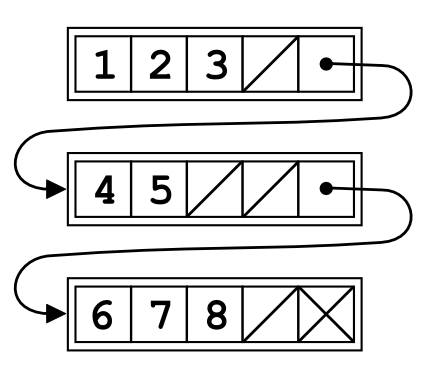
\includegraphics[width=50mm]{unrolled}
\caption{Unrolled linked list}
\label{fig:unrolled}
\end{figure}

Para o caso do radix sort, pelo fato de ter um vetor em cada nó, teria que ocorrer comutações de elementos, e isso pode 
ser custoso. O exemplo acima tem como nó um vetor com capacidade para 4 elementos e um ponteiro para o próximo nó.

%------------------------------------------------

\section{Considerações finais}

Quando se deseja ordenar um certo dado, sempre temos alguma informação sobre esse dado, e através dessa informação 
podemos escolher qual algoritmo de ordenação mais apropriado a utilizar. 
Um outro fator importante na escolha é saber o quanto de memória e tempo está disponível para a execução 
do algoritmo.
Na computação é comum ouvirmos o termo \emph{trade-off}, que significa \emph{troca}. É exatamente isso que define a 
escolha dos algoritmos. Se é desejado o menor tempo de execução, perderá em memória. Se memória é o problema, então 
perderá no tempo. Ou pode haver um meio termo, consumindo uma quantia de memória e tempo de execução aceitável.

Os algoritmos quadráticos geralmente não são boas escolhas, exceto quando a quantia de dados é pequena ou o tempo de 
processamento não é relevante. Quando os dados estiverem parcialmente ordenados, o insertion sort é uma boa escolha.

Porém, tempo de execução é algo sempre relevante, e o peso da escolha se resume à quanto de memória poderá ser 
cedido ao algoritmo. Em casos onde a memória nunca é o problema ou o valor do maior elemento a ser ordenado for 
pequeno, o rank sort, como comprovado pelos gráficos acima, é a melhor opção.

O problema é que nas aplicações do mundo real, memória e tempo possuem restrições. Um algoritmo que consome o dobro de 
memória necessária para armazenar elementos e não possui um pior caso, tendo complexidade constante, é o merge sort, e 
se o gasto dessa memória extra não for problema, ele é uma boa escolha. 

O algoritmo quick sort, talvez o mais conhecido, não necessita de memória extra e possui bom desempenho, porém no 
pior caso tem desempenho quadrático. Conhecendo a natureza dos dados e fazendo uma boa escolha do pivô, cair no 
pior caso é muito difícil. Quando os dados estiverem bem embaralhados, escolher como pivô o primeiro elemento é suficiente. 
Mas, não sabendo nada sobre os dados, escolher como pivô um elemento aleatório é a melhor saída para não cair no pior caso. 
Para a escolha do elemento resultante da mediana de três como pivô, deve se conhecer os dados, pois se estiverem 
parcialmente ordenados, pode ter um desempenho ruim. A mediana de três pode ser sempre uma boa escolha dependendo 
de como o quick sort for implementado. Para este artigo, o quick sort foi implementado trocando o pivô com o 
primeiro elemento, e depois o colocando em sua posição correta. Se for implementado de maneira que o pivô não seja comutado 
com o primeiro elemento para ordenar os dados e depois retorná-lo à sua posição, a mediana de três não cai no pior caso 
mostrado acima [\ref{mediana}].

O heap sort é um algoritmo de complexidade constante, a mesma do melhor caso do quick sort, não tendo um pior caso. 
Porém não é indicado para grande quantidade de dados, pois faz muitos acessos a partes de memória distantes. Este é, 
novamente, um problema de falha de cache. O quick sort, escolhendo um bom pivô de acordo com a natureza dos dados, é 
uma melhor escolha que o heap sort, pois tira proveito do \emph{Princípio de localidade de referência} [\ref{qsortBest1}]
[\ref{qsortBest2}][\ref{qvsh}].

Quando se trata em ordenar elementos em memória não sequencial, utilizando lista encadeada por exemplo, o radix sort 
é uma boa opção. Porém, se o algoritmo implementado não tiver uma boa técnica para tirar proveito do 
princípio de localidade de referência, o resultado será muito ruim caso os dados estiverem dispostos em uma ordem 
aleatória. Mas no caso da escolha do radix sort, é preferível a versão decimal, pois por mais que o binário 
não possua operações de divisão e sim de \emph{shift} e \emph{and}, o que é menos custoso, ter apenas dois baldes 
demanda mais iterações do algoritmo para obter os dados ordenados. 

Não é seguro comparar algoritmos implementados para estrutura de dados diferente, como o radix sort e o quick sort, 
pois na prática, como já dito, a maneira como esses dados estão organizados na memória é muito relevante.

Abaixo, segue o gráfico do tempo de execução dos algoritmos para a base de 10\textsuperscript{8} números a serem 
ordenados, em ordem aleatória. Os algoritmos que caíram no pior caso tiveram seus dados omitidos.\newline

{\setlength{\parindent}{-0.5em}
\scalebox{0.9}{
\begin{bchart}[max=201, plain, scale=0.9, unit=s]
\bcbar[label=1]{103.221}
\bcbar[label=2]{10.754}
\bcbar[label=3]{60.310}
\bcbar[label=4]{59.992}
\bcbar[label=5]{56.944}
\bcbar[label=6]{59.062}
\bcbar[label=7]{66.290}
\bcbar[label=8]{87.275}
\bcbar[label=9]{95.656}
\bcbar[label=10]{200.753}
\end{bchart}}}

% Do 1 ao 10, respectivamente, shell sort, rank sort, merge sort, quick sort com pivô como: primeiro elemento, elemento 
% central, elemento aleatório, elemento resultante do cálculo da mediana de três, heap sort, radix sort versão decimal e
%  versão binário.
Do 1 ao 10, respectivamente: shell, rank, merge, quick sort com pivô como elemento o: primeiro, central, aleatório, resultante da mediana de três, heap, radix sort decimal e binário.\newline

A resposta de qual o melhor algoritmo de ordenação sempre vai ser: \textbf{depende}. Levando em consideração a 
configuração da máquina que irá executar o algoritmo como, sistema de gerenciamento de memória, tecnologia do processador 
e da memória, uma boa maneira é implementar os algoritmos e executá-los, fazendo um comparativo entre 
a desempenho desses algoritmos nesta máquina. Impotante também, é fazer este comparativo utilizando os dados que 
se deseja ordenar, pois, como já citado, a natureza deles pode influenciar.

Desconsiderando a configuração da máquina, fazendo apenas uma análise matemática dos algoritmos, podemos decidir 
qual utilizar, porém pode ser que ao executá-los, o resultado tenha uma diferença significante, pois como dito, 
depende dos dados e da máquina.

No livro \emph{The Art of Computer Programming} [\ref{stackquick}], no volume 3, \emph{Donald Knuth} mostra uma análise exata de vários 
algoritmos de ordenação para o caso médio. Essa análise foi feita baseada em um computador artificial inventado pelo 
autor, no qual ele se refere como \emph{``a typical computer''}. Segue abaixo a análise dos algoritmos quick sort, merge 
sort, heap sort e insertion sort: 

\begin{itemize}
\item Quick sort: $11.667 \cdot (n + 1) \cdot \log_2(n) - 1.74n - 18.74$
\item Merge sort: $12.5n \cdot \log_2(n)$
\item Heap sort: $16n \cdot \log_2(n) + 0.01n$
\item Insertion sort: $2.25n\textsuperscript{2} + 7.75n - 3\log_2(n)$
\end{itemize}

\begin{figure}[ht]\centering 
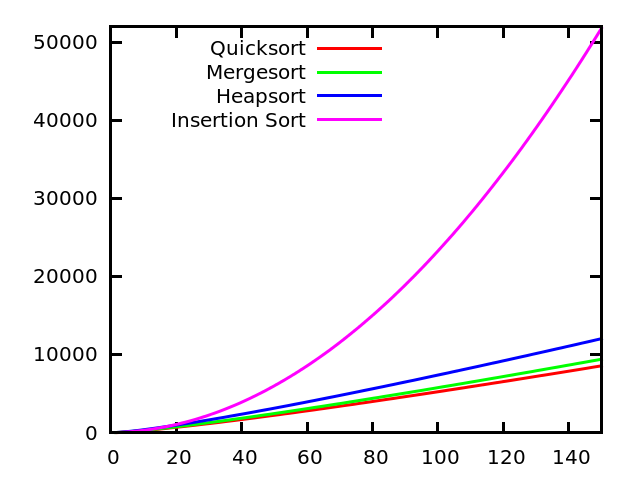
\includegraphics[width=\linewidth]{knuth1}
\caption{Gráfico da análise}
\label{fig:knuth1}
\end{figure}

Esses resultados indicam que o quick sort é o mais rápido. Mas, isso foi provado apenas para a máquina artificial 
do \emph{Knuth}. Isso não implica que o mesmo resultado será obtido para as máquinas reais. Note também que os 
algoritmos se relacionam de maneira diferente para pequenas entradas:

\begin{figure}[ht]\centering 
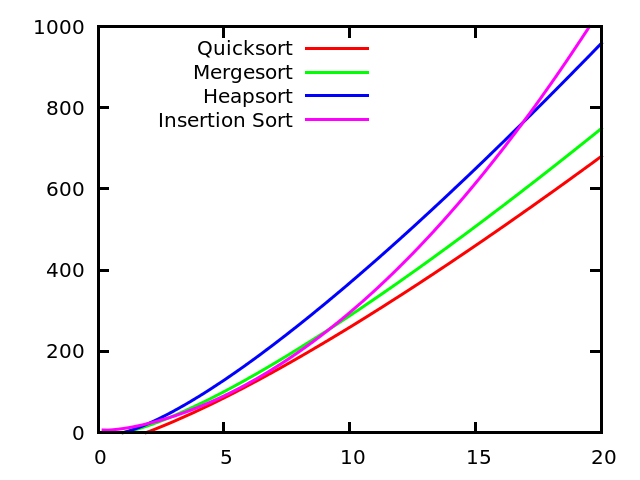
\includegraphics[width=\linewidth]{knuth2}
\caption{Gráfico da análise para pequenas entradas}
\label{fig:knuth2}
\end{figure}

%----------------------------------------------------------------------------------------
%	REFERENCE LIST
%----------------------------------------------------------------------------------------
%\newpage

%REFERÊNCIAS BIBLIOGRÁFICAS:
\section{Referências Bibliográficas}
\begin{adjustwidth}{}{3cm}
\begin{enumerate}
\item \url{https://en.wikipedia.org/wiki/Sorting_algorithm}\label{SortAlgoWiki}
\item \url{https://en.wikipedia.org/wiki/Shellsort#Gap_sequences}\label{ShellWiki}
\item \url{http://stackoverflow.com/questions/33928819/the-radix-sort-algorithm-may-have-different-run-time-for-datas-with-different-or}\label{Question}
\item \url{http://bigocheatsheet.com/} 
\item \url{https://en.wikipedia.org/wiki/Bubble_sort} 
\item \url{http://www.ufpa.br/sampaio/curso_de_estdados_2/aula2_2.htm} 
\item \url{http://rosettacode.org/wiki/Sorting_algorithms/Insertion_sort#C} 
\item \url{http://rosettacode.org/wiki/Sorting_algorithms/Shell_sort#C} 
\item \url{http://rosettacode.org/wiki/Sorting_algorithms/Selection_sort#C} 
\item \url{http://rosettacode.org/wiki/Sorting_algorithms/Merge_sort#C} 
\item \url{http://www.geeksforgeeks.org/iterative-quick-sort/} 
\item \url{http://www.ime.usp.br/~pf/algoritmos/aulas/quick.html} 
\item \url{https://pt.wikipedia.org/wiki/Heapsort} 
\item \url{http://cs.stackexchange.com/questions/18945/best-and-worse-case-inputs-for-heap-sort-and-quick-sort}\label{Heap}
\item \url{http://stackoverflow.com/questions/1853208/quicksort-superiority-over-heap-sort}\label{qsortBest1}
\item \url{http://stackoverflow.com/questions/4289024/why-is-quicksort-faster-in-average-than-others}\label{qsortBest2}
\item \url{http://stackoverflow.com/questions/2467751/quicksort-vs-heapsort}\label{qvsh}
\item \url{http://cs.stackexchange.com/questions/3/why-is-quicksort-better-than-other-sorting-algorithms-in-practice}\label{stackquick}
\item \url{http://pt.slideshare.net/shimulsakhawat/counting-sortnon-comparison-sort} 
\item \url{http://www.geeksforgeeks.org/counting-sort/} 
\item \url{https://pt.wikipedia.org/wiki/Radix_sort}
\item \url{https://www.cs.usfca.edu/~galles/visualization/RadixSort.html}
\item \url{http://tex.stackexchange.com/} 
\item \url{http://stackoverflow.com/} 
\item \url{http://www.sorting-algorithms.com/} 
\end{enumerate}
\end{adjustwidth}
%----------------------------------------------------------------------------------------

\end{document}

% \begin{algorithm}
% \SetAlgoLined
% \KwData{this text}
% \KwResult{how to write algorithm with \LaTeX2e}
% initialization\;
% \While{not at end of this document}{
% read current\;
% \eIf{understand}{
% go to next section\;
% current section becomes this one\;
% }{
% go back to the beginning of current section\;
% }
% }
% \caption{How to write algorithms}
% \end{algorithm}

 % \begin{algorithm}
 %   \SetAlgoLined
 %   \Entrada{$S,\eta, U$}
 %   \Saida{Número esperado de nodos atingidos}
 %   \Inicio{
   
 %   \Enqto{$n \neq 0$}
 %   {
 %      $\sigma(S) = 0$ \\
 %   }



 %   $\sigma(S) = 0$ \\
 %    \ParaCada{$u \in S$}{
 %   $\sigma(S)\leftarrow \sigma(S)+\textsc{Backtrack}(u,\eta,W,U)$\\
 %     }
 %   }
 %   \Retorna{$\sigma(S)$}
 %   \label{alg1}
 %   \caption{\textsc{Esperança}}
 % \end{algorithm}